\chapter{METODOLOGI}

% Ubah konten-konten berikut sesuai dengan isi dari metodologi

\section{Desain Sistem}
\label{sec:desainsistem}

Judul untuk tugas akhir “Sistem Pendeteksi Penggunaan Alat Pelindung Diri (APD) Pada Pekerja Konstruksi” ini berada dalam bidang computer vision atau visi komputer yang memiliki tujuan merancang sistem yang dapat mendeteksi penggunaan Alat Pelindung Diri (APD) secara real-time. Menggunakan YOLOv7 yang merupakan algoritma deteksi objek yang berbasis CNN (Convolutional Neural Network). Dataset yang digunakan berupa gambar-gambar personel proyek yang mengenakan Alat Pelindung Diri (APD) dan yang tidak. Gambar - gambar tersebut dikumpulkan dari beberapa sumber seperti dataset dari penelitian sebelumnya dan sumber lainnya.

\begin{figure}[ht]
  \centering
  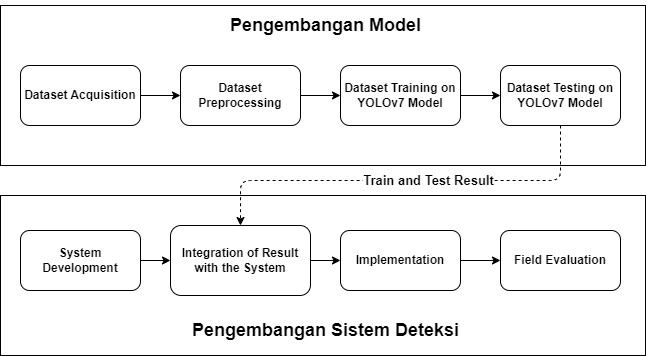
\includegraphics[width=1.0\textwidth]{gambar/desain_sistem.png}
  \caption{Bagan Umum Sistem}
  \label{fig:baganumumsistem}
\end{figure}

\newpage

\section{Akuisisi Dataset}
\label{sec:akuisisidataset}

Dataset yang digunakan untuk training menggunakan YOLOv7 berupa dataset berisi gambar - gambar yang mengandung personel lapangan proyek yang mengenakan Alat Pelindung Diri (APD) dan yang tidak mengenakan APD. Untuk penelitian ini, dataset yang digunakan bersumber dari:

\subsection{CHVG Dataset oleh Md. Ferdous dan Sk. Md. Masudul Ahsan}
\label{chvgdataset}

\par Dataset ini merupakan dataset yang dibuat dan digunakan pada penelitian oleh Md. Ferdous dan Sk. Md. Masudul Ahsan pada bulan Juni tahun 2022 tentang sistem pendeteksi APD.
CHVG merupakan singkatan dari \textit{Color Hardhat, Vest, Glass} yang menggambarkan konten dari dataset itu sendiri. Dataset ini berisi delapan kelas yang berbeda, yaitu helm keselamatan kerja 4 warna (merah, biru, kuning, dan putih) dimana setiap warna memiliki kelasnya sendiri, rompi, kacamata pengaman, tubuh orang, dan kepala orang.
Dataset ini berisi 1.699 gambar dengan ukuran 640x640 dan anotasi yang sesuai dari delapan kelas tersebut \cite{Ferdous2022}.

\begin{figure}[ht]
  \centering
  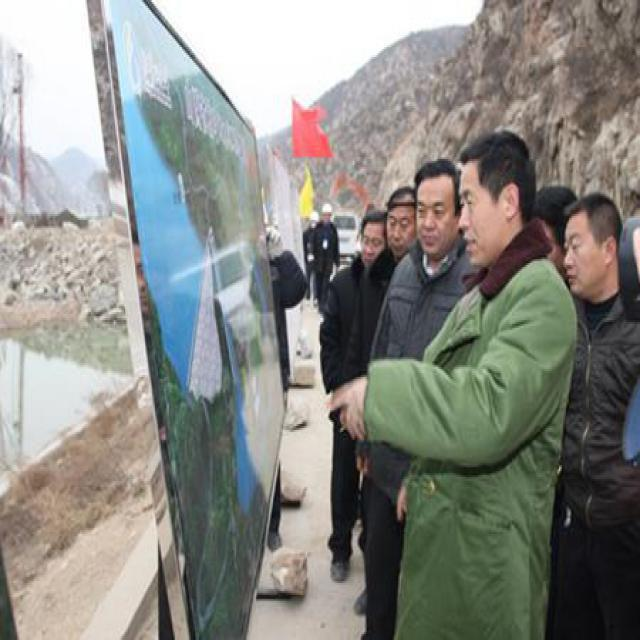
\includegraphics[width=0.3\textwidth]{gambar/chvg1}
  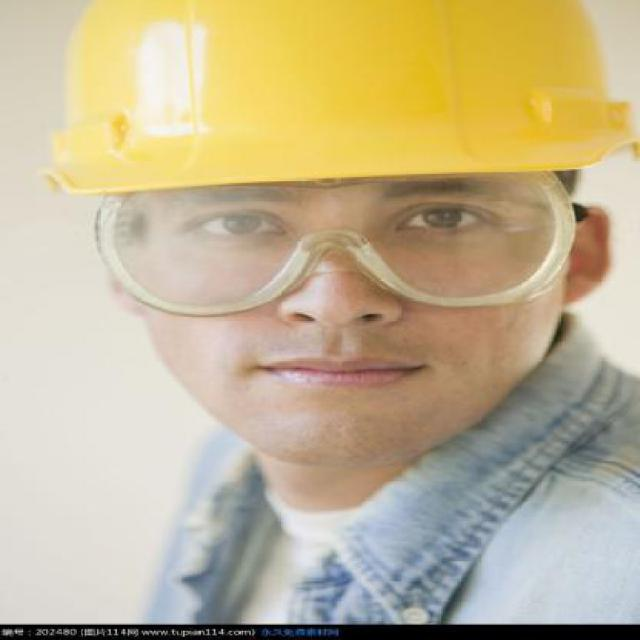
\includegraphics[width=0.3\textwidth]{gambar/chvg2}
  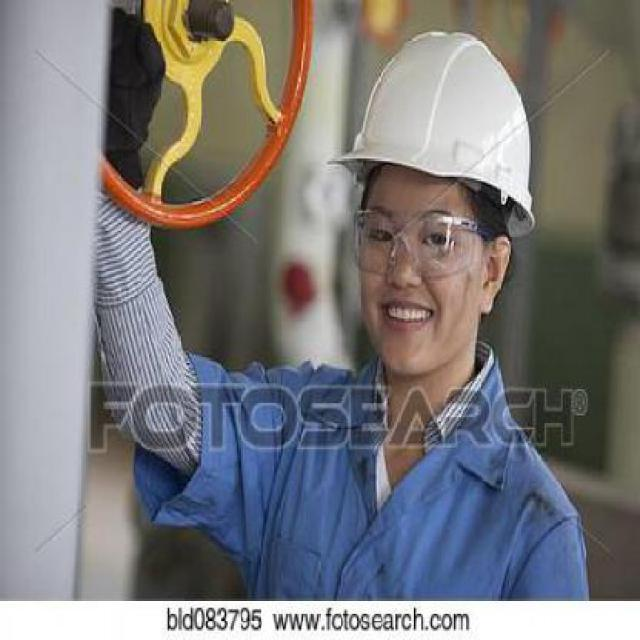
\includegraphics[width=0.3\textwidth]{gambar/chvg3}
  \caption{Sampel gambar pada CHVG Dataset oleh Md. Ferdous dan Sk. Md. Masudul Ahsan}
  \label{fig:datasetapdpreview}
\end{figure}

\subsection{Roboflow Universe Open Source Dataset}
\label{roboflowdataset}

Penulis mengambil 2 macam dataset dari platform Roboflow Universe yaitu "Gloves Data- set" dan "Boots Dataset". Kedua dataset tersebut merupakan dataset yang disediakan secara open source oleh platform Roboflow yang dapat digunakan secara umum karena sifatnya yang \emph{open source}. Sesuai namanya, kedua dataset tersebut berisi gambar sarung tangan dan sepatu keselamatan kerja yang sesuai dengan ketentuan APD. Dataset ini memiliki 3 kelas yaitu glove, safety boot, dan worker yang sudah dianotasikan dengan sesuai. Dataset ini memiliki total 894 gambar dengan resolusi 1920x1080 \cite{gloves-7zhos_dataset} \cite{boots-uzihq_dataset}.

\section{\textit{Preprocessing} Dataset}
\label{sec:preprocessing}
\par Ada beberapa proses yang dilakukan untuk dataset yang sudah dikumpulkan agar bisa digunakan untuk proses training dengan benar. Proses tersebut meliputi membersihkan dataset, augmentasi gambar, dan pembagian dataset. Untuk penelitian ini, proses - proses tersebut akan dilakukan pada platform Roboflow.

\section{Training dan Testing Model YOLOv7}
\label{sec:trainingdataset}

\par Dataset - dataset yang sudah di pre-process sebelumnya di roboflow dan sudah memiliki anotasi yang sesuai lalu digunakan untuk training model menggunakan algoritma YOLOv7. Training ini merupakan proses pelatihan model dengan input gambar - gambar dari dataset yang sudah diberi anotasi dimana gambar dan anotasinya tersebut diolah hingga menghasilkan suatu karakteristik atau pola khusus dari kelas/label yang ditentukan sebelumnya lewat anotasi sehingga selanjutnya dapat digunakan komputer untuk menebak gambar yang nantinya dideteksi. Karena YOLOv7 yang menggunakan PyTorch sebagai framework machine learningnya, hasil training nya berupa bobot atau weight yang akan diexport dalam bentuk .pt (format pytorch).

\par Hasil training model YOLOv7 tersebut kemudian dilakukan testing dengan cara melakukan proses \textit{inference} dimana input gambar yang digunakan merupakan gambar-gambar dari dataset itu sendiri yang sebelumnya digunakan untuk proses training.

\section{Pengembangan Sistem}
\label{sec:pengembangansistem}

Sistem deteksi Alat Pelindung Diri (APD) ini akan memanfaatkan YOLOv7 untuk melaku- kan prediksi pada input yang diterima. Input berupa gambar yang diterima dari
webcam atau camera yang terhubung ke komputer yang akan menjalankan sistem ini.
Sistem dikembangkan dengan tujuan untuk mendeteksi penggunaan Alat Pelindung Diri (APD) secara real-time dan akan menjalankan mekanisme alarm jika pada camera input
terdapat seseorang yang tidak menggunakan Alat Pelindung Diri (APD) secara lengkap. Dalam hal ini yaitu menggunakan helm, kacamata, dan rompi.

Sistem akan dibuat dalam bentuk file script python yang dapat dijalankan pada device komputer atau laptop. Script ini akan menerima beberapa parameter input yang dibutuhkan untuk menjalankan prediksi dengan model YOLOv7. Parameter input yang dibutuhkan yaitu salah satunya input feed camera dari webcam yang digunakan atau bisa dalam bentuk file gambar atau video.
Selain itu user akan harus memberikan parameter-parameter lain secara manual yang dibutuhkan model YOLOv7 agar dapat bisa menjalankan prediksi. Setelah semua parameter telah dipenuhi, sistem akan memberikan output berupa \textit{bounding box} yang meng-\textit{highlight} komponen-komponen APD yang ada pada gambar.

\section{Integrasi Sistem dengan Hasil Training Model}
\label{subsec:integrasi}

Sistem deteksi yang sudah dikembangkan akan diintegrasikan dengan model YOLOv7 yang sudah dilakukan training dan testing menggunakan CHVG dataset. Setelah diintegrasikan, sistem akan siap untuk diimplementasikan secara real-time dengan memanfaatkan input dari kamera webcam.

\section{Implementasi}
\label{subsec:implementasi}

Sistem deteksi yang sudah dilakukan integrasi selanjutnya akan diimplementasikan dimana sistem digunakan pada kondisi \textit{real-time}. Kamera webcam akan diarahkan kepada orang yang menggunakan maupun tidak menggunakan Alat Pelindung Diri (APD). Proses ini dilakukan berulang kali dengan beberapa variabel yang berbeda contohnya seperti kondisi gelap, berkabut, dan hujan.

\section{Evaluasi}
\label{subsec:evaluasi}

Setelah sistem deteksi diimplementasikan secara \emph{real-time} dengan beberapa variabel yang berbeda, dilakukan analisa hasil sebagai evaluasi sistem dan penelitian secara kesuluruhan. Setiap hasil dari variabel-variabel yang diuji akan dibandingkan untuk setiap jenis percobaan.

\section{Bahan dan peralatan yang digunakan}
\label{subsec:peralatan}

Dalam penelitian ini, bahan dan peralatan yang akan digunakan dalam rangka menyelesaikan penelitian ini mulai dari tools berupa software atau perangkat lunak hingga hardware atau perangkat keras. Berikut pemaparan dari alat-alat yang digunakan.

\begin{enumerate}[nolistsep]
  \item Computer Desktop
  \item Google Colab
  \item Webcam Papalook PA552pro
\end{enumerate}

\begin{longtable}{|c|c|c|}
  \caption{Spesifikasi Komputer Desktop}
  \label{tb:spesifikasikomputer}                         \\
  \hline
  % \rowcolor[HTML]{C0C0C0}
  \textbf{Tipe}      & \textbf{Detail}                   \\
  \hline
  \textit{Processor} & AMD Ryzen 3 3300X                 \\
  Memory             & 16 GB                             \\
  Storage            & HDD 1TB SSD 512GB                 \\
  Graphic Card       & NVIDIA GeForce GTX 1650 Super 4GB \\
  Operating System   & Windows 11                        \\
  CUDA               & CUDA version 11.8                 \\
  \hline
\end{longtable}

\begin{longtable}{|c|c|c|}
  \caption{Spesifikasi Webcam Papalook PA552pro}
  \label{tb:spesifikasiwebcam}                           \\
  \hline
  % \rowcolor[HTML]{C0C0C0}
  \textbf{Tipe} & \textbf{Detail}                        \\
  \hline
  Resolution    & 1920x1080                              \\
  Max FPS       & 60 FPS                                 \\
  Other Detail  & Full 360 Degree Rotation               \\
                & Auto Focus                             \\
                & Auto Exposure White Balance            \\
                & 3 Level Lighting Adjustable Ring Light \\
  \hline
\end{longtable}

\section{Urutan pelaksanaan penelitian}

Alur waktu penelitian yang akan dilaksanakan akan mengacu pada tabel yang ditunjukkan pada Tabel~\ref{tb:timeline}.

% Ubah tabel berikut sesuai dengan isi dari rencana kerja
\newcommand{\w}{}
\newcommand{\G}{\cellcolor{gray}}
\begin{table}[h!]
  \caption{\emph{Timeline} Penelitian}
  \label{tb:timeline}

  \begin{tabular}{|p{3.5cm}|c|c|c|c|c|c|c|c|c|c|c|c|c|c|c|c|}
    \hline
    \multirow{2}{*}{Kegiatan} & \multicolumn{16}{|c|}{Minggu}                                                                       \\
    \cline{2-17}              &
    1                         & 2                             & 3  & 4  & 5  & 6  & 7  & 8  & 9  & 10 & 11 & 12 & 13 & 14 & 15 & 16 \\
    \hline

    % Gunakan \G untuk mengisi sel dan \w untuk mengosongkan sel
    Studi Literatur           &
    \G                        & \G                            & \G & \G & \w & \w & \w & \w & \w & \w & \w & \w & \w & \w & \w & \w \\
    \hline

    Pengolahan Data           &
    \w                        & \w                            & \G & \G & \G & \G & \w & \w & \w & \w & \w & \w & \w & \w & \w & \w \\
    \hline

    Training dan Testing      &
    \w                        & \w                            & \w & \w & \w & \G & \G & \G & \G & \w & \w & \w & \w & \w & \w & \w \\
    \hline

    Pengembangan Sis- tem     &
    \w                        & \w                            & \w & \w & \G & \G & \G & \G & \G & \w & \w & \w & \w & \w & \w & \w \\
    \hline

    Integrasi Sistem          &
    \w                        & \w                            & \w & \w & \w & \w & \w & \w & \w & \G & \G & \w & \w & \w & \w & \w \\
    \hline

    Implementasi              &
    \w                        & \w                            & \w & \w & \w & \w & \w & \w & \w & \w & \w & \G & \G & \G & \G & \w \\
    \hline

    Evaluasi                  &
    \w                        & \w                            & \w & \w & \w & \w & \w & \w & \w & \w & \w & \w & \w & \w & \G & \G \\
    \hline

    Pembuatan Laporan         &
    \G                        & \G                            & \G & \G & \G & \G & \G & \G & \G & \G & \G & \G & \G & \G & \G & \G \\
    \hline
  \end{tabular}
\end{table}